% !TeX root = ../../thesis.tex

\subsection{\tcp{}}
Both \acrshort{tsm} and \acrshort{tcs} attempt to execute as few tests as possible to reduce the execution time of the test suite. Nevertheless, in some cases, we may require to execute every test case to guarantee correctness. In this situation, we can still optimise the test suite. \acrfull{tcp} aims to find a permutation of the sequence of test cases, rather than eliminating specific tests from being executed (\Cref{fig:tcp}). We choose the order of the permutation in such a way that we can complete a predefined objective as soon as possible. Once we have achieved our objective, we can early terminate the execution of the test suite. In the worst-case scenario, we will still execute every test case. Some examples of objectives include covering as many lines of code as fast as possible or executing tests ordered on their probability of failure \cite{10.1002/stv.430}. \Cref{def:tcp} provides a formal definition of this approach.

\begin{definition}[\tcp{}]
\label{def:tcp}
\mbox{}\\Given:
\begin{itemize}
	\item $T$ the test suite.
	\item $PT$ the set of permutations of $T$.
	\item $f: PT \mapsto \mathbb{R}$ a function which is used to compare sequences of test cases to find the optimal permutation.
\end{itemize}

\noindent \tcp{} finds a permutation $T' \in PT$ such that $\forall T'' \in PT : f(T') \ge f(T'') \Rightarrow (T'' \ne T')$ 
\end{definition}

\begin{figure}[htbp!]
	\centering
	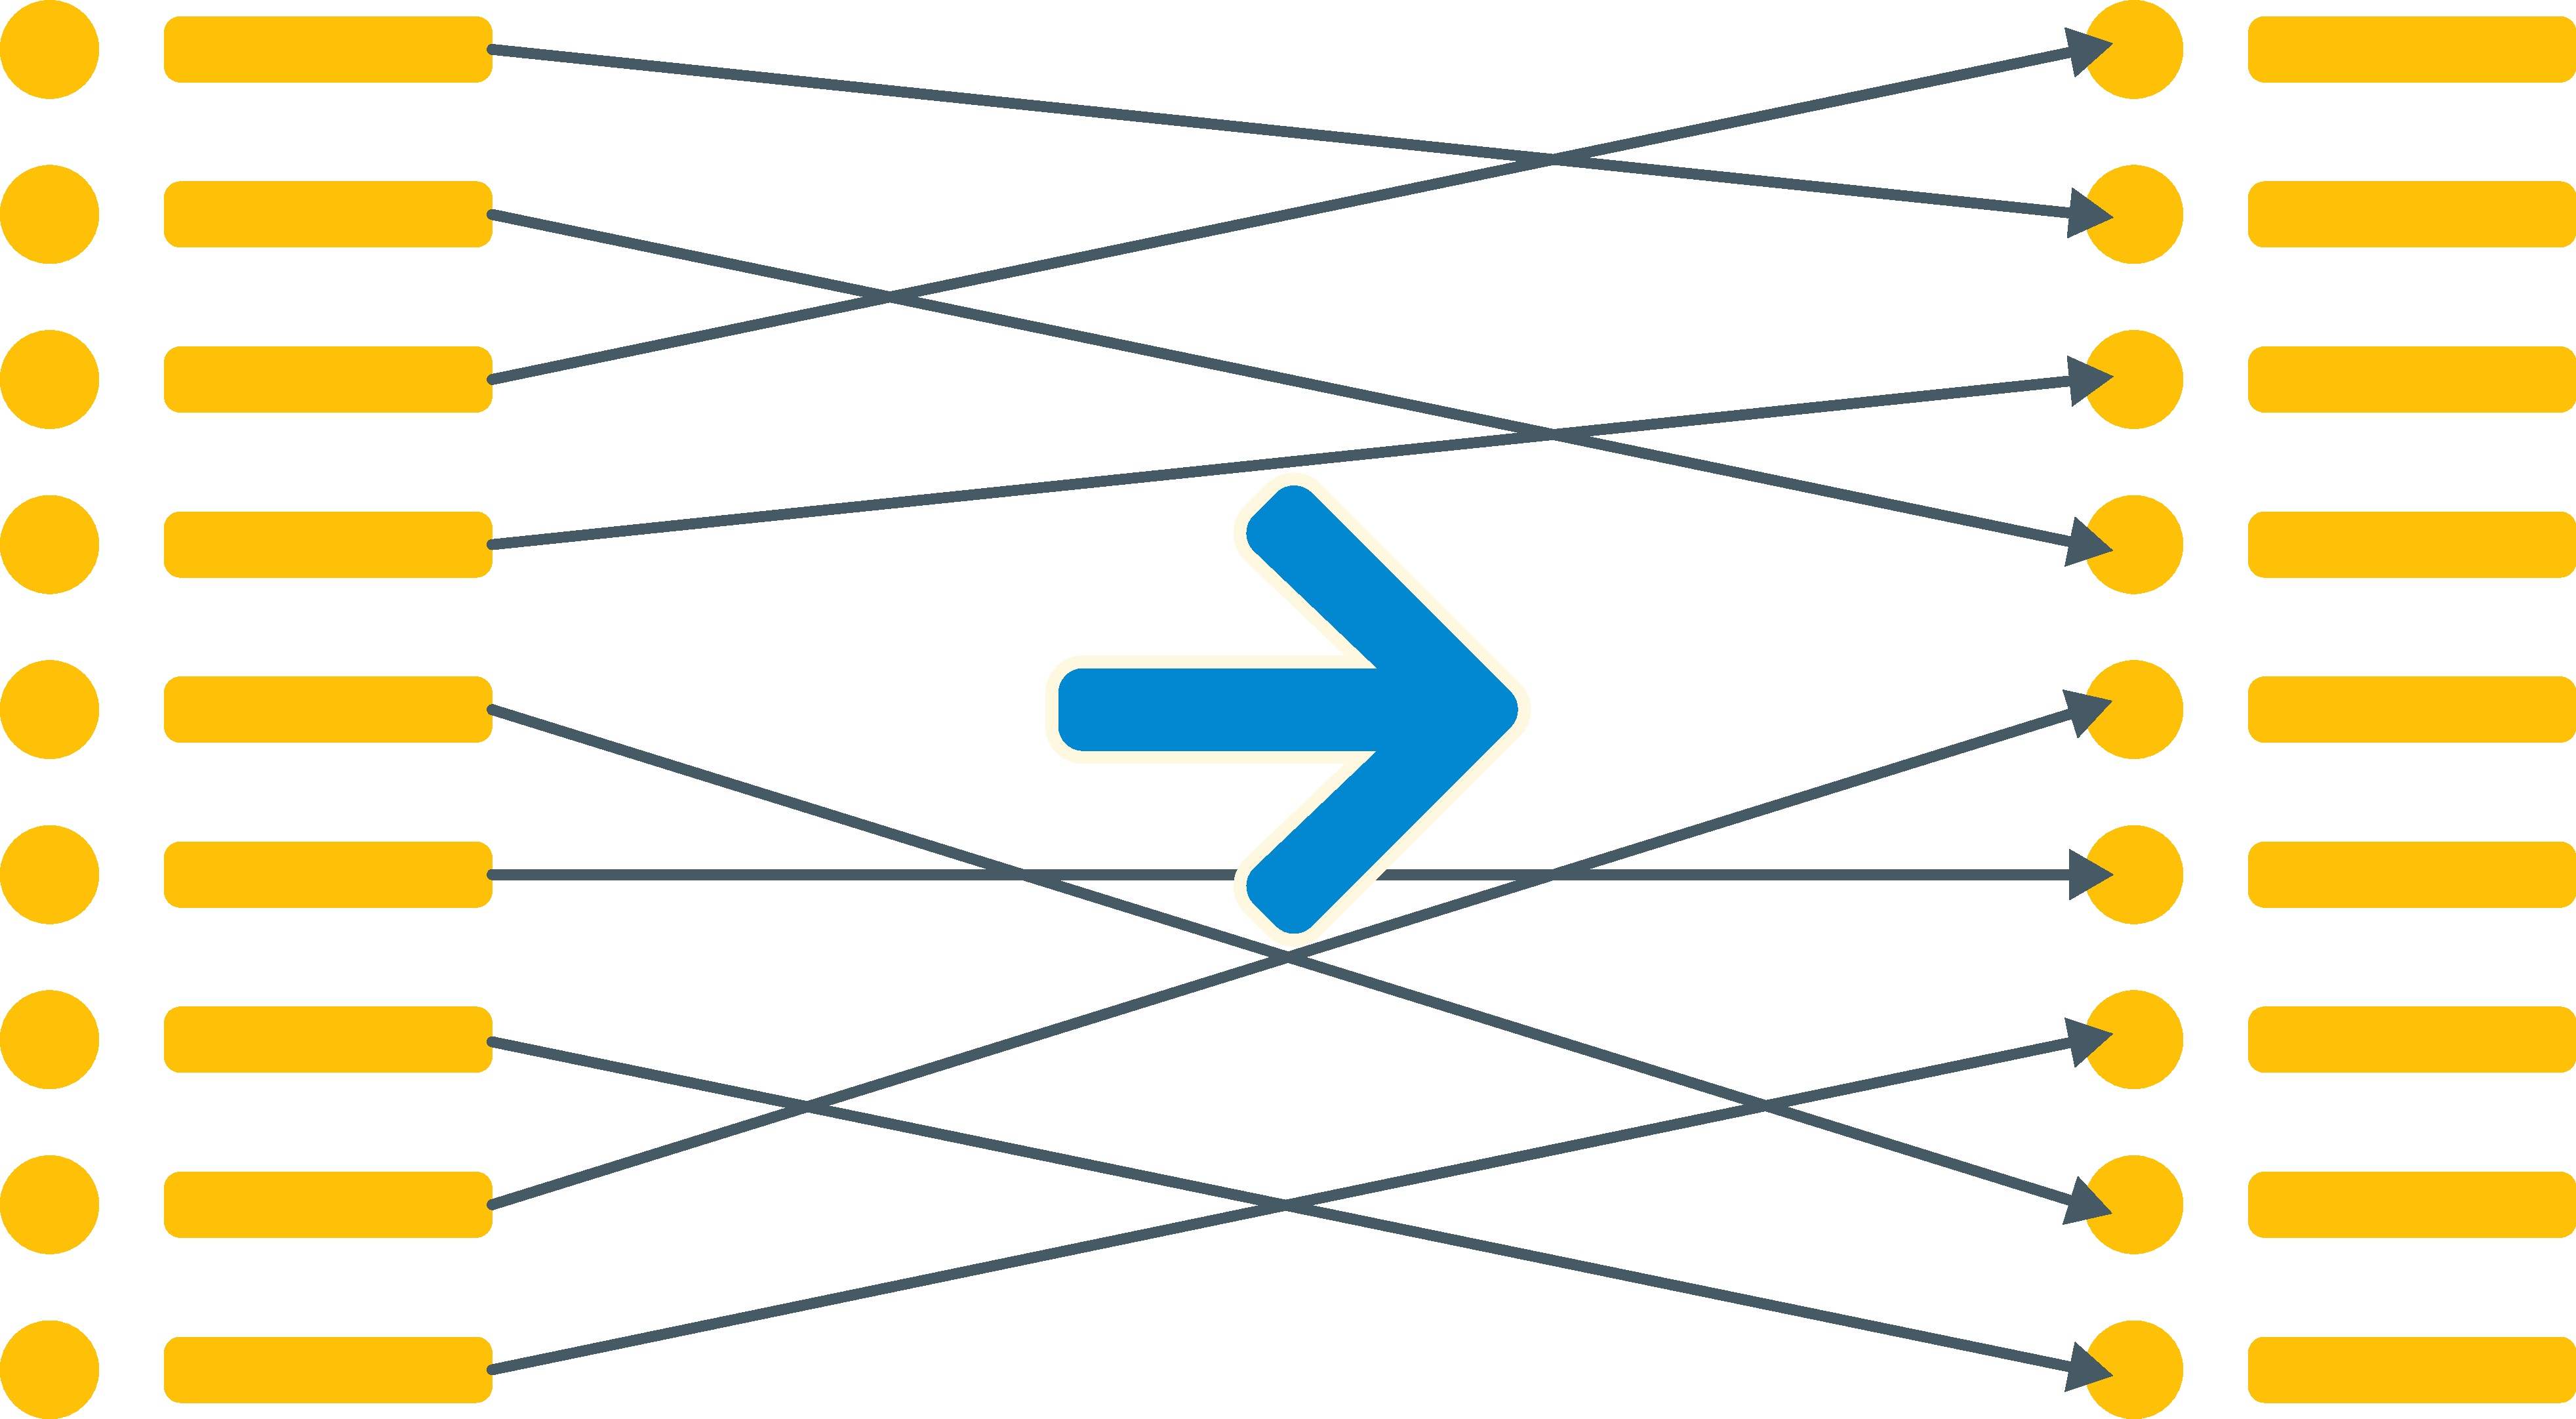
\includegraphics[width=\textwidth]{assets/tikz/approach-tcp.tikz}
	\caption{\tcp{}.}
	\label{fig:tcp}
\end{figure}